\documentclass{beamer}

\newcommand{\lesson}{Review 2: Object-Oriented Programming}


\newcommand{\course}{Introduction to Object-Oriented Programming}
\subject{\course}
\title[\lesson]{\course}
\subtitle{\lesson}

\author[CS 1331]
{Christopher Simpkins \\\texttt{chris.simpkins@gatech.edu}}
\institute[Georgia Tech]

\date[]{}

\newcommand{\link}[2]{\href{#1}{\textcolor{blue}{\underline{#2}}}}
\newcommand{\code}{http://www.cs1331.org/code}

\usepackage{colortbl}

% If you have a file called "university-logo-filename.xxx", where xxx
% is a graphic format that can be processed by latex or pdflatex,
% resp., then you can add a logo as follows:

% \pgfdeclareimage[width=0.6in]{coc-logo}{cc_2012_logo}
% \logo{\pgfuseimage{coc-logo}}

\mode<presentation>
{
  \usetheme{Berlin}
  \useoutertheme{infolines}

  % or ...

 \setbeamercovered{transparent}
  % or whatever (possibly just delete it)
}

\usepackage{tikz}
% Optional PGF libraries
\usepackage{pgflibraryarrows}
\usepackage{pgflibrarysnakes}
\usepackage{pgfplots}
\usepackage{fancybox}
\usepackage{listings}
\usepackage{hyperref}
\hypersetup{colorlinks=true,urlcolor=blue}
\usepackage[english]{babel}
% or whatever

\usepackage[latin1]{inputenc}
% or whatever

\usepackage{times}
\usepackage[T1]{fontenc}
% Or whatever. Note that the encoding and the font should match. If T1
% does not look nice, try deleting the line with the fontenc.


\usepackage{listings}

% "define" Scala
\lstdefinelanguage{scala}{
  morekeywords={abstract,case,catch,class,def,%
    do,else,extends,false,final,finally,%
    for,if,implicit,import,match,mixin,%
    new,null,object,override,package,%
    private,protected,requires,return,sealed,%
    super,this,throw,trait,true,try,%
    type,val,var,while,with,yield},
  otherkeywords={=>,<-,<\%,<:,>:,\#,@},
  sensitive=true,
  morecomment=[l]{//},
  morecomment=[n]{/*}{*/},
  morestring=[b]",
  morestring=[b]',
  morestring=[b]""",
}

\usepackage{color}
\definecolor{dkgreen}{rgb}{0,0.6,0}
\definecolor{gray}{rgb}{0.5,0.5,0.5}
\definecolor{mauve}{rgb}{0.58,0,0.82}

% Default settings for code listings
\lstset{frame=tb,
  language=scala,
  aboveskip=2mm,
  belowskip=2mm,
  showstringspaces=false,
  columns=flexible,
  basicstyle={\scriptsize\ttfamily},
  numbers=none,
  numberstyle=\tiny\color{gray},
  keywordstyle=\color{blue},
  commentstyle=\color{dkgreen},
  stringstyle=\color{mauve},
  frame=single,
  breaklines=true,
  breakatwhitespace=true,
  keepspaces=true
  %tabsize=3
}


% If you wish to uncover everything in a step-wise fashion, uncomment
% the following command:

% \beamerdefaultoverlayspecification{<+->}

\begin{document}

\begin{frame}
  \titlepage
\end{frame}

%------------------------------------------------------------------------
\begin{frame}[fragile]{Topics in the OOP Block}


\begin{itemize}
\item Inheritance
\item Polymorphism
\item Abstract classes
\item Interfaces
\item The {\tt equals(Object)} method
\item Overriding versus Overloading
\item Enums
\item Exceptions
\end{itemize}


\end{frame}
%------------------------------------------------------------------------

%------------------------------------------------------------------------
\begin{frame}[fragile]{Inheritance and Polymorphism}


Consider
\begin{lstlisting}[language=Java]
public abstract class Animal { public abstract void speak(); }
public class Mammal extends Animal {
    public void speak() { System.out.println("Hello!"); }
}
public class Dog extends Mammal {
    public void speak() { System.out.println("Woof, woof!"); }
    public void wagTail() { System.out.println("(wags tail)"); }
}
public class Cat extends Mammal {
    public void speak() { System.out.println("Meow!"); }
}
\end{lstlisting}

We'll use these classes in the examples in the remaining slides.

\end{frame}
%------------------------------------------------------------------------

%------------------------------------------------------------------------
\begin{frame}[fragile]{Assignments}


A reference variable has a compile-time type, and refers to an object which has a run-time type.
\begin{itemize}
\item The type of the {\it l-value} (to the left of the {\tt =} symbol) in an assignment statement is the compile-time type
\item The type of the {\it r-value} (to the right of the {\tt =} symbol) in an assignment statement is the run-time type
\item For reference assignments the type of the {\it r-value} must be a subclass of the type of the {\it l-value}
\item Remember that every class is a subclass of itself.
\end{itemize}

So this is fine:
\begin{lstlisting}[language=Java]
Animal fido = new Dog();
\end{lstlisting}
But this is not:
\begin{lstlisting}[language=Java]
Dog spot = new Mammal();  // Error: Mammal not a subclass of Dog
\end{lstlisting}


\end{frame}
%------------------------------------------------------------------------

%------------------------------------------------------------------------
\begin{frame}[fragile]{Casting and Method Binding}


Casting affects compile-time types (some would say ``casting shuts the compiler up'') but method binding is always based on run-time types.  So
\begin{lstlisting}[language=Java]
Dog fido = new Dog();
((Mammal) fido).speak();
\end{lstlisting}
Produces
\begin{lstlisting}[language=bash]
Woof, woof!
\end{lstlisting}
Even though {\tt Mammal}s say ``Hello!'' because the run-time type of {\tt spot} is still {\tt Dog}.

\end{frame}
%------------------------------------------------------------------------

%------------------------------------------------------------------------
\begin{frame}[fragile]{Upcasting and Downcasting}


The assignment statements we've seen so far are examples of implicit upcasting.
\begin{itemize}
\item Upcasting means treating a reference as an instance of one of its superclasses.
\item Upcasting is safe becuase every object contains the elements of each of its superclasses.
\item Downcasting means treating a reference as an instance of one of its subclasses
\item Downcasting is not safe in general because subclasses may add methods not present in superclasses.  This is why Java doesn't implicitly downcast in assignment statements.
\end{itemize}
Think of upcasting as ``going up'' the class hierarchy and downcasting as ``going down'' the class hierarchy.


\end{frame}
%------------------------------------------------------------------------

%------------------------------------------------------------------------
\begin{frame}[fragile]{Upcasting and Downcasting Examples}


Consider the following:
\begin{lstlisting}[language=Java]
1: Mammal mittens = (Mammal) new Cat(); // Safe
2: Mammal sparky = new Mammal();
3: // Compiles, but will cause a ClassCastException at run-time,
4: Dog huh = (Dog) sparky;
5: // so we won't even get here.
6: huh.wagTail();
\end{lstlisting}

\begin{itemize}
\item The upcast in line 1 is fine.
\item The downcast in line 4 will compile but will cause a {\tt ClassCastException} at run-time.
\item We won't even get to line 6 due to the exception, which is good because a mammal doesn't have a {\tt wagTail} method.  This is what the {\tt ClassCastException} is guarding against.
\end{itemize}


\end{frame}
%------------------------------------------------------------------------

%------------------------------------------------------------------------
\begin{frame}[fragile]{Java's Exception Hierarchy}

\begin{columns}[t]
\begin{column}{2in}
\begin{center}
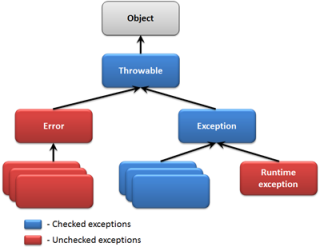
\includegraphics[height=2.5in]{hierarchy_of_java_exceptions.png}
\end{center}
\end{column}
\begin{column}{3in}
\begin{itemize}
\item Most (checked) exceptions will subclass {\tt Exception}
\item Most uncheked exceptions will subclass {\tt RuntimeException}
\item {\tt Error} is for compiler hackers.  Don't use it directly.
\end{itemize}
\end{column}
\end{columns}

\end{frame}
%------------------------------------------------------------------------


%------------------------------------------------------------------------
\begin{frame}[fragile]{Catch or Declare}

\vspace{-.05in}
Checked exceptions, sublcasses of {\tt Throwable} that are not subclasses of {\tt RuntimeException}, must be caught or propagated:\\
\vspace{.05in}
Catch:
\vspace{-.05in}
\begin{lstlisting}[language=Java,escapechar=`]
public Company(String employeeDataFile) {
  // ...
  try {
    employees = initFromFile(new File(employeeDataFile));
  } `\colorbox{yellow}{catch (FileNotFoundException e) \{}`
    System.out.println(e.getMessage());
  }
}
\end{lstlisting}
\vspace{-.05in}
Declare (propagating the exception):
\vspace{-.05in}
\begin{lstlisting}[language=Java,escapechar=`]
public Company(String employeeDataFile) `\colorbox{yellow}{throws FileNotFoundException \{}`
  // ...
  initFromFile(new File(employeeDataFile));
}
\end{lstlisting}
\vspace{-.05in}
Propagating an exception unwinds the stack of methods that led to the point where the exception was thrown.
\end{frame}
%------------------------------------------------------------------------

%------------------------------------------------------------------------
\begin{frame}[fragile]{Exceptions Question}

\vspace{-.05in}
\begin{lstlisting}[language=Java]
public class A extends Throwable { ... }
public class B extends A { ... }
public class C extends RuntimeException { ... }
\end{lstlisting}
\vspace{-.05in}
Which of the following methods will {\bf not} compile?
\vspace{-.05in}
\begin{enumerate} \itemsep0pt

\item
\begin{lstlisting}[language=Java]
    A foo(B b) throws C {
        if (true) throw new C("c");
        return new B("b");
    }
\end{lstlisting}

\item
\begin{lstlisting}[language=Java]
    A bar(B b) throws C {
        if (true) throw new RuntimeException("c");
        return new B("c");
    }
\end{lstlisting}

\item
\begin{lstlisting}[language=Java]
    A baz(B b) throws B {
        if (true) throw new A("a");
        return new B("c");
    }
\end{lstlisting}


\end{enumerate}


\end{frame}
%------------------------------------------------------------------------

%------------------------------------------------------------------------
\begin{frame}[fragile]{Exceptions Question - Answer}

\vspace{-.05in}
\begin{lstlisting}[language=Java]
public class A extends Throwable { ... }
public class B extends A { ... }
public class C extends RuntimeException { ... }
\end{lstlisting}
\vspace{-.05in}
Which of the following methods will {\bf not} compile?
\vspace{-.05in}
\begin{enumerate} \itemsep0pt
\item
\begin{lstlisting}[language=Java]
    A foo(B b) throws C {
        if (true) throw new C("c");
        return new B("b");
    }
\end{lstlisting}

\item
\begin{lstlisting}[language=Java]
    A bar(B b) throws C {
        if (true) throw new RuntimeException("c");
        return new B("c");
    }
\end{lstlisting}

\item This won't compile because {\tt A} is not a subclass of {\tt B}.
\begin{lstlisting}[language=Java]
    A baz(B b) throws B {
        if (true) throw new A("a");
        return new B("c");
    }
\end{lstlisting}


\end{enumerate}



\end{frame}
%------------------------------------------------------------------------


%------------------------------------------------------------------------
\begin{frame}[fragile]{Override Equivalence}

Two methods are \href{http://docs.oracle.com/javase/specs/jls/se8/html/jls-8.html#jls-8.4.2}{override-equivalent} if:
\begin{itemize}
\item they have the same name,
\item they have the same parameter lists, and
\item their return values are \link{http://docs.oracle.com/javase/tutorial/java/javaOO/returnvalue.html}{covariant}
\end{itemize}

\end{frame}
%------------------------------------------------------------------------


%------------------------------------------------------------------------
\begin{frame}[fragile]{Override Equivalence Question}

Given the following classes:

\begin{lstlisting}[language=Java]
public class A { ... }
public class B extends A { ... }
public class C extends A { ... }
\end{lstlisting}

and the method signature:

\begin{lstlisting}[language=Java]
public A foo(B b);
\end{lstlisting}

Which of the following method signatures is override eqivalent?

\begin{enumerate}
\item {\tt public B foo(A bar)}
\item {\tt public C foo(B bar)}
\item {\tt public C foo(B bar)}
\item {\tt public B foo(C bar)}
\end{enumerate}


\end{frame}
%------------------------------------------------------------------------

%------------------------------------------------------------------------
\begin{frame}[fragile]{Override Equivalence Question - Answer}

Given the following classes:

\begin{lstlisting}[language=Java]
public class A { ... }
public class B extends A { ... }
public class C extends A { ... }
\end{lstlisting}

and the method signature:

\begin{lstlisting}[language=Java]
public A foo(B b);
\end{lstlisting}

Which of the following method signatures is override eqivalent?

\begin{enumerate}
\item {\tt public B foo(A bar)}
\item {\tt {\bf public C foo(B bar)}}
\item {\tt public C foo(B bar)}
\item {\tt public B foo(C bar)}
\end{enumerate}


\end{frame}
%------------------------------------------------------------------------

% %------------------------------------------------------------------------
% \begin{frame}[fragile]{}


% \begin{lstlisting}[language=Java]

% \end{lstlisting}

% \begin{itemize}
% \item
% \end{itemize}


% \end{frame}
% %------------------------------------------------------------------------


\end{document}
